% !TeX document-id = {7d4b2264-2136-4f1e-938f-66e1e0753aeb}
% !TEX TS-program = XeLaTeX
% Commands for running this example:
% 	 xelatex main
% 	 bibtex8 -W -c cp1256fa main
%      xindy -L persian -C utf8 -M texindy main
% 	 xelatex main
% 	 xelatex main
% End of Commands

%        نمونه پایان‌نامه آماده شده با استفاده از کلاس IUST-Thesis، نگارش 0.6
% 		محمود امین‌طوسی، دانشگاه تربیت معلم سبزوار، http://profsite.sttu.ac.ir/mamintoosi/
% 		گروه پارسی‌لاتک  http://www.parsilatex.com
%        این نسخه، بر اساس نسخه‌ 0.4 از کلاس Tabriz_Thesis آقای وحید دامن‌افشان آماده شده است. http://damanafshan.tk
%        
%        تغییرات:
%        نسخه 0.6:
%        اصلاح مشکل بسته subfig 
%        اگر قصد نوشتن پروژه کارشناسی را دارید، در خط زیر به جای msc، کلمه bsc و اگر قصد نوشتن پروژه دکترا
%        را دارید، کلمه phd را قرار دهید. کلیه تنظیمات لازم، به طور خودکار، اعمال می‌شود.

%        اگر مایلید پایان‌نامه شما دورو باشد به جای oneside  در خط زیر از twoside استفاده کنید
\documentclass[oneside,openany,msc]{IUST-Thesis}
% مشخصات پایان‌نامه را در فایلهای faTitle و enTitle وارد نمایید.
%       فایل commands.tex را مطالعه کنید؛ چون دستورات مربوط به فراخوانی بسته زی‌پرشین 
%       و دیگر بسته‌ها و ... در این فایل قرار دارد و بهتر است که با نحوه استفاده از آنها آشنا شوید.
% در این فایل، دستورها و تنظیمات مورد نیاز، آورده شده است.
%-------------------------------------------------------------------------------------------------------------------

% در ورژن جدید زی‌پرشین برای تایپ متن‌های ریاضی، این سه بسته، حتماً باید فراخوانی شود
\usepackage{amsthm,amssymb,amsmath}
% بسته‌ای برای تنطیم حاشیه‌های بالا، پایین، چپ و راست صفحه
\usepackage[top=40mm, bottom=40mm, left=25mm, right=35mm]{geometry}
% بسته‌‌ای برای ظاهر شدن شکل‌ها و تصاویر متن
\usepackage{graphicx}
% بسته‌ای برای رسم کادر
\usepackage{framed} 
% بسته‌‌ای برای چاپ شدن خودکار تعداد صفحات در صفحه «معرفی پایان‌نامه»
\usepackage{lastpage}
% بسته‌ و دستوراتی برای ایجاد لینک‌های رنگی با امکان جهش
\usepackage[pagebackref=false,colorlinks,linkcolor=blue,citecolor=blue]{hyperref}
% چنانچه قصد پرینت گرفتن نوشته خود را دارید، خط بالا را غیرفعال و  از دستور زیر استفاده کنید چون در صورت استفاده از دستور زیر‌‌، 
% لینک‌ها به رنگ سیاه ظاهر خواهند شد که برای پرینت گرفتن، مناسب‌تر است
%\usepackage[pagebackref=false]{hyperref}
% بسته‌ لازم برای تنظیم سربرگ‌ها
\usepackage{fancyhdr}
%
\usepackage{setspace}
\usepackage{algorithm}
\usepackage{algorithmic}
\usepackage{subfigure}
\usepackage[subfigure]{tocloft}


% بسته‌ای برای ظاهر شدن «مراجع» و «نمایه» در فهرست مطالب
\usepackage[nottoc]{tocbibind}
% دستورات مربوط به ایجاد نمایه
\usepackage{makeidx}
\makeindex
%%%%%%%%%%%%%%%%%%%%%%%%%%
% فراخوانی بسته زی‌پرشین و تعریف قلم فارسی و انگلیسی
\usepackage[extrafootnotefeatures]{xepersian}
\settextfont[Scale=1]{XBNiloofar.ttf}
\setlatintextfont[Scale=0.9]{Times New Roman}

%%%%%%%%%%%%%%%%%%%%%%%%%%
% چنانچه می‌خواهید اعداد در فرمول‌ها، انگلیسی باشد، خط زیر را غیرفعال کنید
\setdigitfont[Scale=1]{XBZar.ttf}%{Persian Modern}
%%%%%%%%%%%%%%%%%%%%%%%%%%
% تعریف قلم‌های فارسی و انگلیسی اضافی برای استفاده در بعضی از قسمت‌های متن
\defpersianfont\titlefont[Scale=1]{XBNiloofar.ttf}
% \defpersianfont\iranic[Scale=1.1]{XB Zar Oblique}%Italic}%
% \defpersianfont\nastaliq[Scale=1.2]{IranNastaliq}

%%%%%%%%%%%%%%%%%%%%%%%%%%
% دستوری برای حذف کلمه «چکیده»
\renewcommand{\abstractname}{}
% دستوری برای حذف کلمه «abstract»
%\renewcommand{\latinabstract}{}
% دستوری برای تغییر نام کلمه «اثبات» به «برهان»
\renewcommand\proofname{\textbf{برهان}}
% دستوری برای تغییر نام کلمه «کتاب‌نامه» به «مراجع»
\renewcommand{\bibname}{مراجع}
% دستوری برای تعریف واژه‌نامه انگلیسی به فارسی
\newcommand\persiangloss[2]{#1\dotfill\lr{#2}\\}
% دستوری برای تعریف واژه‌نامه فارسی به انگلیسی 
\newcommand\englishgloss[2]{#2\dotfill\lr{#1}\\}
% تعریف دستور جدید «\پ» برای خلاصه‌نویسی جهت نوشتن عبارت «پروژه/پایان‌نامه/رساله»
\newcommand{\پ}{پروژه/پایان‌نامه/رساله }

%\newcommand\BackSlash{\char`\\}

%%%%%%%%%%%%%%%%%%%%%%%%%%
\SepMark{-}

% تعریف و نحوه ظاهر شدن عنوان قضیه‌ها، تعریف‌ها، مثال‌ها و ...
\theoremstyle{definition}
\newtheorem{definition}{تعریف}[section]
\theoremstyle{theorem}
\newtheorem{theorem}[definition]{قضیه}
\newtheorem{lemma}[definition]{لم}
\newtheorem{proposition}[definition]{گزاره}
\newtheorem{corollary}[definition]{نتیجه}
\newtheorem{remark}[definition]{ملاحظه}
\theoremstyle{definition}
\newtheorem{example}[definition]{مثال}

%\renewcommand{\theequation}{\thechapter-\arabic{equation}}
%\def\bibname{مراجع}
\numberwithin{algorithm}{chapter}
\def\listalgorithmname{فهرست الگوریتم‌ها}
\def\listfigurename{فهرست تصاویر}
\def\listtablename{فهرست جداول}

%%%%%%%%%%%%%%%%%%%%%%%%%%%%
% دستورهایی برای سفارشی کردن سربرگ صفحات
% \newcommand{\SetHeader}{
% \csname@twosidetrue\endcsname
% \pagestyle{fancy}
% \fancyhf{} 
% \fancyhead[OL,EL]{\thepage}
% \fancyhead[OR]{\small\rightmark}
% \fancyhead[ER]{\small\leftmark}
% \renewcommand{\chaptermark}[1]{%
% \markboth{\thechapter-\ #1}{}}
% }
%%%%%%%%%%%%5
%\def\MATtextbaseline{1.5}
%\renewcommand{\baselinestretch}{\MATtextbaseline}
\doublespacing
%%%%%%%%%%%%%%%%%%%%%%%%%%%%%
% دستوراتی برای اضافه کردن کلمه «فصل» در فهرست مطالب

\newlength\mylenprt
\newlength\mylenchp
\newlength\mylenapp

\renewcommand\cftpartpresnum{\partname~}
\renewcommand\cftchappresnum{\chaptername~}
\renewcommand\cftchapaftersnum{:}

\settowidth\mylenprt{\cftpartfont\cftpartpresnum\cftpartaftersnum}
\settowidth\mylenchp{\cftchapfont\cftchappresnum\cftchapaftersnum}
\settowidth\mylenapp{\cftchapfont\appendixname~\cftchapaftersnum}
\addtolength\mylenprt{\cftpartnumwidth}
\addtolength\mylenchp{\cftchapnumwidth}
\addtolength\mylenapp{\cftchapnumwidth}

\setlength\cftpartnumwidth{\mylenprt}
\setlength\cftchapnumwidth{\mylenchp}	

\makeatletter
{\def\thebibliography#1{\chapter*{\refname\@mkboth
   {\uppercase{\refname}}{\uppercase{\refname}}}\list
   {[\arabic{enumi}]}{\settowidth\labelwidth{[#1]}
   \rightmargin\labelwidth
   \advance\rightmargin\labelsep
   \advance\rightmargin\bibindent
   \itemindent -\bibindent
   \listparindent \itemindent
   \parsep \z@
   \usecounter{enumi}}
   \def\newblock{}
   \sloppy
   \sfcode`\.=1000\relax}}
\makeatother


\begin{document}

\pagenumbering{harfi}
% !TeX root=main.tex
% در این فایل، عنوان پایان‌نامه، مشخصات خود، متن تقدیمی‌، ستایش، سپاس‌گزاری و چکیده پایان‌نامه را به فارسی، وارد کنید.
% توجه داشته باشید که جدول حاوی مشخصات پروژه/پایان‌نامه/رساله و همچنین، مشخصات داخل آن، به طور خودکار، درج می‌شود.
%%%%%%%%%%%%%%%%%%%%%%%%%%%%%%%%%%%%
% دانشگاه خود را وارد کنید
\university{علم و صنعت ایران}
% دانشکده، آموزشکده و یا پژوهشکده  خود را وارد کنید
\faculty{دانشکده مهندسی کامپیوتر}
% گروه آموزشی خود را وارد کنید
\department{گروه هوش مصنوعی و رباتیک}
% گروه آموزشی خود را وارد کنید
\subject{مهندسی کامپیوتر}
% گرایش خود را وارد کنید
\field{هوش مصنوعی و رباتیک}
% عنوان پایان‌نامه را وارد کنید
\title{نوشتن پروژه، پایان‌نامه و رساله با استفاده از کلاس 
IUST-Thesis}
% نام استاد(ان) راهنما را وارد کنید
\firstsupervisor{استاد راهنمای اول}
\secondsupervisor{استاد راهنمای دوم}
% نام استاد(دان) مشاور را وارد کنید. چنانچه استاد مشاور ندارید، دستور پایین را غیرفعال کنید.
\firstadvisor{استاد مشاور اول}
%\secondadvisor{استاد مشاور دوم}
% نام دانشجو را وارد کنید
\name{محمود}
% نام خانوادگی دانشجو را وارد کنید
\surname{امین‌طوسی}
% شماره دانشجویی دانشجو را وارد کنید
\studentID{87922012}
% تاریخ پایان‌نامه را وارد کنید
\thesisdate{اسفند ۱۳۹۰}
% به صورت پیش‌فرض برای پایان‌نامه‌های کارشناسی تا دکترا به ترتیب از عبارات «پروژه»، «پایان‌نامه» و »رساله» استفاده می‌شود؛ اگر  نمی‌پسندید هر عنوانی را که مایلید در دستور زیر قرار داده و آنرا از حالت توضیح خارج کنید.
%\projectLabel{پایان‌نامه}

% به صورت پیش‌فرض برای عناوین مقاطع تحصیلی کارشناسی تا دکترا به ترتیب از عبارات «کارشناسی»، «کارشناسی ارشد» و »دکترا» استفاده می‌شود؛ اگر  نمی‌پسندید هر عنوانی را که مایلید در دستور زیر قرار داده و آنرا از حالت توضیح خارج کنید.
%\degree{}

\firstPage
\besmPage
\davaranPage

%\vspace{.5cm}
% در این قسمت اسامی اساتید راهنما، مشاور و داور باید به صورت دستی وارد شوند
%\renewcommand{\arraystretch}{1.2}
\begin{center}
\begin{tabular}{| p{8mm} | p{18mm} | p{.17\textwidth} |p{14mm}|p{.2\textwidth}|c|}
\hline
ردیف	& سمت & نام و نام خانوادگی & مرتبه \newline دانشگاهی &	دانشگاه یا مؤسسه &	امضـــــــــــــا\\
\hline
۱  &	استاد راهنما				 & دکتر \newline محمود فتحی & دانشیار & دانشگاه \newline علم و صنعت ایران &  \\
\hline
۲ &     استاد مشاور				 & دکتر \newline ناصر مزینی & استادیار & دانشگاه \newline علم و صنعت ایران & \\
\hline
۳ &      استاد مدعو\newline  خارجی			 & دکتر \newline محمدحسن \newline قاسمیان & استاد & دانشگاه \newline تربیت مدرس & \\
\hline
۴ &	استاد مدعو\newline  خارجی			 & دکتر \newline  نصرالله مقدم & استادیار & دانشگاه \newline  تربیت مدرس& \\
\hline
۵ &	استاد مدعو\newline  داخلی			 & دکتر\newline  رضا برنگی & استادیار & دانشگاه \newline  علم و صنعت ایران & \\
\hline
۶ &	استاد مدعو\newline  داخلی			 & دکتر\newline  محسن سریانی & استادیار & دانشگاه \newline  علم و صنعت ایران & \\
\hline
۷ &	استاد مدعو\newline  داخلی			 &دکتر \newline محمدرضا جاهدمطلق & دانشیار& دانشگاه \newline  علم و صنعت ایران & \\
\hline
\end{tabular}
\end{center}

\esalatPage
\mojavezPage


% چنانچه مایل به چاپ صفحات «تقدیم»، «نیایش» و «سپاس‌گزاری» در خروجی نیستید، خط‌های زیر را با گذاشتن ٪  در ابتدای آنها غیرفعال کنید.
 % پایان‌نامه خود را تقدیم کنید!

 \newpage
\thispagestyle{empty}
{\Large تقدیم به:}\\
\begin{flushleft}
{\huge
همسر و فرزندانم\\
\vspace{7mm}
و\\
\vspace{7mm}
پدر و مادرم
}
\end{flushleft}


% سپاس‌گزاری
\begin{acknowledgementpage}
سپاس خداوندگار حکیم را که با لطف بی‌کران خود، آدمی را زیور عقل آراست.


در آغاز وظیفه‌  خود  می‌دانم از زحمات بی‌دریغ استاد  راهنمای خود،  جناب آقای دکتر ...، صمیمانه تشکر و  قدردانی کنم  که قطعاً بدون راهنمایی‌های ارزنده‌  ایشان، این مجموعه  به انجام  نمی‌رسید.

از جناب  آقای  دکتر ...   که زحمت  مطالعه و مشاوره‌  این رساله را تقبل  فرمودند و در آماده سازی  این رساله، به نحو احسن اینجانب را مورد راهنمایی قرار دادند، کمال امتنان را دارم.

همچنین لازم می‌دانم از پدید آورندگان بسته زی‌پرشین، مخصوصاً جناب آقای  وفا خلیقی، که این پایان‌نامه با استفاده از این بسته، آماده شده است و همه دوستانمان در گروه پارسی‌لاتک کمال قدردانی را داشته باشم.

 در پایان، بوسه می‌زنم بر دستان خداوندگاران مهر و مهربانی، پدر و مادر عزیزم و بعد از خدا، ستایش می‌کنم وجود مقدس‌شان را و تشکر می‌کنم از خانواده عزیزم به پاس عاطفه سرشار و گرمای امیدبخش وجودشان، که بهترین پشتیبان من بودند.
% با استفاده از دستور زیر، امضای شما، به طور خودکار، درج می‌شود.
\signature 
\end{acknowledgementpage}
%%%%%%%%%%%%%%%%%%%%%%%%%%%%%%%%%%%%
% کلمات کلیدی پایان‌نامه را وارد کنید
\keywords{زی‌پرشین، لاتک، قالب پایان‌نامه، الگو}
%چکیده پایان‌نامه را وارد کنید، برای ایجاد پاراگراف جدید از \\ استفاده کنید. اگر خط خالی دشته باشید، خطا خواهید گرفت.
\fa-abstract{
این پایان‌نامه، به بحث در مورد نوشتن پروژه، پایان‌نامه و رساله با استفاده از کلاس 
\lr{IUST-Thesis}
می‌پردازد.
حروف‌چینی پروژه کارشناسی، پایان‌نامه یا رساله یکی از موارد پرکاربرد استفاده از زی‌پرشین است. 
زی‌پرشین بسته‌ای است که به همت آقای وفا خلیقی آماده شده است و امکان حروف‌چینی فارسی در \lr{\LaTeXe}{} را  برای فارسی‌زبانان فراهم کرده است.
از جمله مزایای لاتک آن است که در صورت وجود یک کلاس آماده برای حروف‌چینی یک سند خاص مانند یک پایان‌نامه، کاربر بدون درگیری با جزییات حروف‌چینی و صفحه‌آرایی می‌تواند سند خود را آماده نماید.
\\
شاید با قالب‌های لاتکی که برخی از مجلات برای مقالات خود عرضه می‌کنند مواجه شده باشید. اگر نظیر این کار در دانشگاههای مختلف برای اسناد متنوع آنها مانند پایا‌ن‌نامه‌ها آماده شود، دانشجویان به جای وقت گذاشتن روی صفحه‌آرایی مطالب خود، روی محتوای متن خود تمرکز خواهند نمود. به علاوه با آشنایی با لاتک خواهند توانست از امکانات بسیار این نرم‌افزار جهت نمایش بهتر دست‌آوردهای خود استفاده کنند.
به همین خاطر، یک کلاس با نام 
\lr{IUST-Thesis}
 برای حروف‌چینی پروژه‌ها، پایان‌نامه‌ها و رساله‌های دانشگاه علم و صنعت ایران با استفاده از نرم‌افزار زی‌پرشین،  آماده شده است. این فایل به 
گونه‌ای طراحی شده است که کلیات خواسته‌های مورد نیاز  مدیریت تحصیلات تکمیلی دانشگاه علم و صنعت ایران را برآورده می‌کند و نیز، حروف‌چینی بسیاری از قسمت‌های آن، به طور خودکار انجام می‌شود.
}

%\fa-abstract{
%%این پایان‌نامه، به بحث در مورد نوشتن پروژه، پایان‌نامه و رساله با استفاده از کلاس 
%%\lr{IUST-Thesis}
%%می‌پردازد. 
%%حروف‌چینی پروژه کارشناسی، پایان‌نامه یا رساله یکی از موارد پرکاربرد استفاده از زی‌پرشین است. 
%%زی‌پرشین بسته‌ای است که به همت آقای وفا خلیقی آماده شده است و امکان حروف‌چینی فارسی در  را  برای فارسی‌زبانان فراهم کرده است.
%%از جمله مزایای لاتک آن است که در صورت وجود یک کلاس آماده برای حروف‌چینی یک سند خاص مانند یک پایان‌نامه، کاربر بدون درگیری با جزییات حروف‌چینی و صفحه‌آرایی می‌توان سند خود را آماده نماید.
%
%شاید با قالب‌های لاتکی که برخی از مجلات برای مقالات خود عرضه می‌کنند مواجه شده باشید. اگر نظیر این کار در دانشگاههای مختلف برای اسناد متنوع آنها مانند پایا‌ن‌نامه‌ها آماده شود، دانشجویان به جای وقت گذاشتن روی صفحه‌آرایی مطالب خود، روی محتوای متن خود تمرکز خواهند نمود. به علاوه با آشنایی با لاتک خواهند توانست از امکانات بسیار این نرم‌افزار جهت نمایش بهتر دستآوردهای خود استفاده کنند.
%به همین خاطر، یک کلاس با نام 
%\lr{IUST-Thesis}
% برای حروف‌چینی پروژه‌ها، پایان‌نامه‌ها و رساله‌های دانشگاه علم و صنعت ایران با استفاده از نرم‌افزار زی‌پرشین،  آماده شده است. این فایل به 
%گونه‌ای طراحی شده است که کلیات خواسته‌های مورد نیاز  مدیریت تحصیلات تکمیلی دانشگاه علم و صنعت ایران را برآورده می‌کند و نیز، حروف‌چینی بسیاری از قسمت‌های آن، به طور خودکار انجام می‌شود.
%}

\abstractPage

\newpage\clearpage
\tableofcontents \newpage
\listoffigures \newpage

\pagestyle{fancy}
% !TeX root=main.tex
% دستور زیر باید در اولین فصل شما باشد. آن را حذف نکنید!
\pagenumbering{arabic}

\chapter{مقدمه}
\thispagestyle{empty}
یکی از نیازهای اساسی انسان‌ها نیاز به برقراری ارتباط با دیگران و اجتماعی شدن است. پایه ای‌ترین ارتباطات اجتماعی را می‌توان خانواده، بستگان، دوستان و همکاران دانست که روابط معناداری بین افراد در این گروه‌ها برقرار است. این در حالی است که در سال‌های اخیر فناوری دیجیتال و اینترنت شکل جدیدی از ارتباط را تعریف کرده‌اند و در حال حاضر شاهد گسترش بی سابقه شبکه‌های اجتماعی
\LTRfootnote{Social Networks}
 در بین مردم هستیم. به گونه‌ای که اکنون شبکه‌های اجتماعی جزئی از زندگی روزمره مردم شده‌است. 
 
 شبکه‌های اجتماعی به کاربرانش این فرصت را می‌دهد تا آراء و نظرات خود را با دیگران مطرح کنند و از نظرات مختلف مطلع شوند. در سایت‌های خرید وارد شوند و کالای موردنظر خود را جستجو کنند و نظرات خریداران قبلی را بخوانند و سفارش خود را ثبت کنند. به‌راحتی اطلاعات مقصد و هر آنچه برای یک سفر لازم است را از اینترنت دریافت کرده و از نظرات و راهنمایی‌های افرادی که قبلاً این سفر را تجربه کرده‌اند استفاده کنند و با طیب خاطر به سفر بروند. در فعالیت‌های گروهی و تشکل‌های مردم‌نهاد مشارکت کنند. بسیاری از فعالیت‌های این چنینی که ذاتی اجتماعی دارند با کمک اینترنت و ظهور شبکه‌های اجتماعی برای کاربران آسان شده‌اند.
 
در بین همه‌ی این قابلیت‌ها که شبکه‌های اجتماعی کنونی در اختیار ما قرار می‌دهند، شرایطی وجود دارد که این شبکه‌های اجتماعی پاسخگوی نیاز‌های ما نیستند. مثلا بخواهید خبر گم شدن حیوان خانگیتان را در محله‌ی خود اعلام کنید و یا بخواهید یک نردبان قرض بگیرید و یا به دنبال یک دندان‌پزشکی یا لوله‌کش خوب در نزدیکی محل زندگیتان باشید. تمامی این مثال‌ها نیازمند این است که شما با همسایگانتان و افرادی که در نزدیکی شما و محله تان زندگی می کنند؛ در ارتباط باشید. موضوعی که امروزه در زندگی ما کمرنگ شده‌است. از طرفی روند شبکه‌های اجتماعی مثل فیسبوک
\LTRfootnote{Facebook}
، توییتر 
\LTRfootnote{Twitter}
و ... به گونه‌ای است که ما را با دوستانی که 20 سال گذشته با آن‌ها ارتباط داشتیم، متصل می‌کند اما با افرادی که در نزدیکی ما زندگی می‌کنند و نیاز بیشتری به ارتباط با آن‌ها داریم، متصل نمی‌کند.

بنابراین در این پروژه ما قصد داریم که یک شبکه‌ی اجتماعی محلی را پیاده‌سازی کنیم که امکان برقراری ارتباط با همسایگانمان را برای ما ایجاد‌کند. از طرفی چون هدف ما در این شبکه‌ی اجتماعی اتصال به افرادی است که از نظر بعد جغرافیایی به ما نزدیک هستند، می‌توانیم با استفاده از تکنولوژی‌هایی همچون بلوتوث
\LTRfootnote{Bluetooth}
، اتصال نقطه به نقطه وای فای 
\LTRfootnote{Peer to Peer WiFi Connnection}
و ... این ارتباط را حاصل کنیم بدون این که بخواهیم از شبکه‌ی جهانی اینترنت
\LTRfootnote{Internet}
 استفاده کنیم. برای رسیدن به این منظور از شبکه‌ی بی‌سیم مش 
 \LTRfootnote{Wireless Mesh Network}
 نیز استفاده خواهیم کرد. البته لازم به ذکر است که در حالت ایده آل اگر تعداد کاربران این شبکه‌ی اجتماعی مقدار قابل توجه‌ای در سراسر جهان باشد، می‌توان با کاربران دور دست نیز ارتباط برقرار کرد. 

سایر کاربرد‌های این شبکه‌ی اجتماعی به صورت زیر خواهد بود:

\begin{enumerate}
	\item 
	فرض کنید که شما در نزدیکی دانشکده‌ی مهندسی کامپیوتر قرار دارید و یک رویداد در دانشکده‌ی مهندسی کامپیوتر در حال برگزاری است. بنابراین اپلیکیشن به صورت یک اعلان بر روی گوشی شما، برگزاری رویداد را به شما اطلاع رسانی می‌کند.
	\item 
	فرض کنید شما برای روز چهارشنبه، نیاز به کمک کسی دارید که از فرزندتان نگهداری کند. شما می‌توانید درخواست یک پرستار بچه را در این شبکه محلی به اشتراک بگذارید.
	
	\item 
	شما دنبال یک کارواش، مکانیکی یا دندان پزشکی خوب در نزدیکی خانه‌تان هستید. می‌توانید در مورد این موضوعات از دیگران در این شبکه‌ی محلی بپرسید.
	\item 
	فرض کنید که شما دوچرخه‌تان را اطراف خانه تان گم کرده‌اید. می‌توانید این موضوع را در شبکه محلی اعلان کنید تا اگر پیدا شد دیگران به شما در این شبکه‌ی محلی خبر بدهند یا مثلا می‌توانید این موضوع را به عنوان جرم در یک منطقه یا امن نبودن یک محله اعلام کنید.
	
	\item 
	نهاد‌های دولتی می‌توانند در این شبکه عضو بشوند و ساکنین یک محله را از اتفاقاتی مثل آتش‌سوزی، دزدی، خرابی تلفن، قطع آب و گاز و برق و ... مطلع کنند و یا برعکس به این شکل که در صورت اتفاق افتادن هر یک از این حوادث ساکنین آن محله بتوانند در سریع‌ترین زمان ممکن نهاد دولتی مربوطه را مطلع سازند.
	
	\item 
	فرض کنید که یک سازمان مثل هواشناسی در این شبکه محلی عضو شود و مردم یک شهر، روستا یا یک استان را از آب و هوای آن روز با خبر کند. مثلا امروز در مناطق جنوبی شهر آب گرفتگی داریم یا امروز هوا در ساعات  2 تا 3 بعد از ظهر بارانی است؛ لطفا از چتر استفاده کنید.
	
	\item
	شما می‌توانید زمان رفتن به سر کار خود را به بقیه اعلام کنید و اگر کسی از همسایگانتان در مسیر شما قرار داشت، با شما همراه شود.(کاهش ترافیک و آلودگی هوا)
	\item 
	فروشگاه‌ها و هایپرمارکت‌های محله می‌توانند موجودی کالا‌های خود را اعلام کنند و یا تخفیف‌های اقلام مختلف را در این شبکه‌ی محلی قرار بدهند.
	\item 
	می‌توانید از همسایگانتان در خواست اجاره‌ی حیاط، پارکینگ یا خانه شان را برای برگزاری جلسه‌هاو مراسم‌هایتان و ... داشته باشید.
	\item 
	فرض کنید شما نیاز دارید که بسته‌ای را در نزدیکی محدوده‌ی زندگی‌تان ارسال کنید ولی وقت کافی ندارید و می‌توانید در شبکه درخواست کنید که یک نفر به صورت رایگان این کار را برای شما انجام دهد.
	\item 
	می‌توانید در مورد مسائل مختلف محله‌تان رای گیری کنید مثل تغییر نام یک کوچه.
	 
\end{enumerate}
 
\section{کار‌های مربوطه}
\subsection{\lr{Open Garden}}
 \href{https://www.opengarden.com}{\lr{Open Garden}}%
\LTRfootnote{https://www.opengarden.com}
یک سرویس است که این امکان را به مردم می‌دهد که  خدمات اینترنت خود را با افرادی که در نزدیکی آن‌ها هستند؛ به اشتراک بگذارند. بنابراین با استفاده از این دستگاه اشتراک‌گذاری اینترنت، هر کس می‌تواند پهنای باند اضافی اینترنت خود را ارائه دهد و برای آن پول بگیرد یا خدمات اینترنتی را از دیگران خریداری کند.

\subsection{\lr{NextDoor}} 
 \href{https://nextdoor.com}{\lr{NextDoor}}%
\LTRfootnote{https://nextdoor.com/}
یک سرویس شبکه اجتماعی خصوصی برای محله است. این شرکت در سال 2008 در سانفرانسیسکو، کالیفرنیا تاسیس شد و در اکتبر 2011 در ایالات متحده راه اندازی شد. کاربران 
\lr{NextDoor}
نام و نشانی واقعی خود را به وب سایت ارائه می‌دهند. پیام‌های منتشر شده در وب سایت، فقط برای سایر اعضای  
\lr{NextDoor}
در همان محله قابل مشاهده است.
\subsection{\lr{Fire Chat}}
 \href{https://www.opengarden.com/firechat/}{\lr{FireChat}}%
\LTRfootnote{https://www.opengarden.com/firechat/} 
یک برنامه اختصاصی تلفن همراه است که توسط
\lr{Open Garden} 
توسعه داده شده‌است. این شبکه‌ی اجتماعی از شبکه بی‌سیم مش استفاده می‌کند تا تلفن‌های هوشمند بتوانند از طریق بلوتوث، وای فای یا در چارچوب
\lr{Multipeer} 
شرکت اپل بدون اتصال به اینترنت به یکدیگر متصل شوند. همچنین این برنامه این قابلیت را دارد که از طریق اینترنت نیز اتصال برقرار شود.

\lr{FireChat}
به عنوان یک ابزار ارتباطی در برخی اعتراضات مدنی مورد استفاده قرار گرفت؛ اگر چه که برای چنین اهدافی طراحی نشده‌است. از جمله دلایلی که این شبکه‌ی اجتماعی محبوبیت چندانی بین مردم ندارد؛ می‌توان به ضعف در پیاده‌سازی، عدم اتصال مناسب بین دو دستگاه اندورید
\LTRfootnote{Android}
و آیفون
\LTRfootnote{iphone}
، اشکال در عدم ارسال مناسب عکس و غیره اشاره نمود.    
  
\section{جمع‌بندی}
			% فصل اول: مقدمه
% !TeX root=main.tex
\chapter{انتخاب \lr{API}مناسب برای ایجاد ارتباط \lr{Peer to Peer}}
\thispagestyle{empty}

اولین گام برای ساخت یک شبکه‌ی محلی این است که یک 
\lr{API}
موجود یا فناوری موجود را که ارتباط محلی و 
\lr{Peer to Peer}
را برای ما بوجود بیاورد را پیدا کنیم و یا این که از ابتدا قابلیت‌های مورد نیاز را پیاده‌سازی کنیم. بدین منظور چندین 
\lr{API}
شامل
\lr{p2pkit}
\cite{p2pkit}
،
\lr{Alljoyn}
\cite{Alljoyn}
،
\lr{Nearby}
\cite{Nearby}
،
\lr{Hypelabs}
\cite{Hypelabs}
و
\lr{Open Garden}
\cite{OpenGarden} 
را پیدا کردیم.
با این که هر کدام از این 
\lr{API}
ها قابلیت‌های مورد نیاز و اولیه‌ی شبکه‌های اجتماعی را در بردارند، اما مشکل اساسی همه‌ی این 
\lr{API}
ها این است که اپلیکیشنی که بر مبنای این‌ها پیاده‌سازی شده‌باشد، باید به اینترنت متصل باشد تا API بتواند به درستی کار کند. بنابراین از آن جایی که شبکه‌ی اجتماعی ما قرار است بدون اینترنت کار کند، نمی‌توانیم از این 
\lr{API}
ها بهره ببریم.

در ادامه، با فناوری
\lr{WiFi Direct}
 آشنا می‌شویم که بر روی گوشی‌های اندروید موجود است و تمامی قابلیت‌هایی که ما برای برقراری ارتباط محلی گوشی‌ها به یکدیگر را نیاز داریم؛ در خود دارد. با این تفاوت که مشکل 
\lr{API}
ها را هم ندارد و بدون نیاز به اتصال اینترنت می‌تواند کار کند. در ادامه‌ی این فصل به معرفی این فناوری و قابلیت و مزایای آن می‌پردازیم.

\section{فناوری \lr{WiFi Direct}} 
\lr{WiFi Direct}
 فناوری جدید تعریف شده توسط اتحادیه 
\lr{WiFi}
\LTRfootnote{WiFi alliance}
  است که هدف آن ارتقاء ارتباط مستقیم بین دستگاه‌ها است؛ بدون این که به یک نقطه دسترسی بی‌سیم
\LTRfootnote{wireless access point} 
   نیاز باشد.
\lr{WiFi Direct}
بر روی زیر ساخت موفق 
\lr{IEEE 802.11}
بنا شده است و این اجازه را به دستگاه‌ها می‌دهد که در یک ارتباط، یک دستگاه نقش  نقطه دسترسی بی‌سیم را ایفا کند و عملکرد آن را انجام دهد. در حال حاضر می‌توان با استفاده از استاندارد 
\lr{IEEE 802.11}
یک ارتباط مستقیم بین دستگاه‌ها ایجاد کرد. اما اشکالات فراوانی همچون مصرف زیاد انرژی در دستگاه وجود دارد.
\cite{WiFiAlliance}
 
\section{بررسی فنی}
 در یک شبکه معمولی 
\lr{WiFi}
مشتری
\LTRfootnote{client}
 اسکن می‌کند وعضو یکی از شبکه‌های بی‌سیم موجود که توسط نقطه دسترسی بی‌سیم ایجاد و اعلام شده‌است؛ می‌شود. این فرایند در 
\lr{WiFi Direct}
به صورت پویا
\LTRfootnote{dynamic}
انجام می‌شود از این رو یک دستگاه 
\lr{WiFi Direct}
باید هر دو نقش مشتری و نقطه دسترسی بی‌سیم را به طور همزمان اجرا کند.
\cite{WiFiAlliance}

\section{معماری}
دستگاه‌های دارای 
\lr{WiFi Direct}
با ایجاد یک گروه با عنوان 
\lr{P2P Group}
می‌توانند با یکدیگر ارتباط برقرار کنند. دستگاهی که عملکردی همچون نقطه‌ی دسترسی بی‌سیم دارد را 
\lr{P2P Group Owner}
می‌نامند و دستگاهی که در نقش مشتری است را 
\lr{P2P client}
گویند.
هنگامی که یک 
\lr{P2P Group}
ایجاد می‌شود، سایر مشتری‌ها می‌توانند با همان روش سنتی شبکه‌های 
\lr{WiFi}
به گروه بپیوندند. زمانی که یک دستگاه هم در نقش 
\lr{P2P Client}
 و هم در نقش 
\lr{P2P Group Owner}
باشد، دستگاه به طور متناوب با استفاده از اشتراک زمانی 
\LTRfootnote{Time sharing}
بین این دو نقش تغییر می‌کند.(مثال: لپتاپ 2 در بالای شکل \ref{fig:WifiDirectArchitecture})
\cite{WiFiAlliance}

 مانند یک نقطه‌ی دسترسی بی سیم سنتی، یک
\lr{P2P Group Owner}
، خود را از طریق 
\lr{beacons}
  اعلام می‌کند. تنها دستگاهی که 
\lr{P2P Group Owner}
 است؛ قادر است دستگاه‌های متصل در گروه خود را به یک شبکه‌ی خارجی متصل کند.(مثال: موبایل موجود در بالا‌ی شکل \ref{fig:WifiDirectArchitecture}) این ارتباط باید در لایه‌ی شبکه 
\LTRfootnote{Network Layer}
اتفاق بیفتد و معمولا با استفاده از 
\lr{NAT}
\LTRfootnote{Network Address Translation}
پیاده سازی می‌شود.
\lr{WiFi Direct}
اجازه نمی‌دهد که نقش 
\lr{P2P Group Owner}
به افراد دیگری در گروه انتقال یابد.

\begin{figure}
	\centerline{
	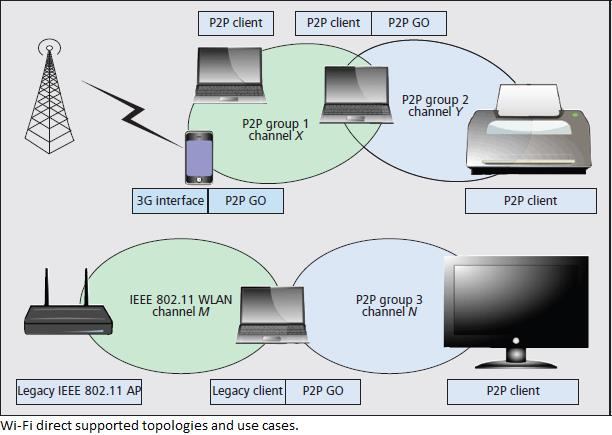
\includegraphics{images/wifidirectarchitecture.jpg}}
	\caption{معماری \lr{Wifi Direct}\cite{Camps-Mur}}
	\label{fig:WifiDirectArchitecture}
\end{figure}

\section{تشکیل گروه}
سه نوع روش برای تشکیل گروه در فناوری
\lr{WiFi Direct}
وجود دارد که عبارتند از استاندار
\LTRfootnote{Standard}
،مستقل
\LTRfootnote{Autonomus}
و پایدار
\LTRfootnote{Persistent}
.

تشکیل گروه شامل دو مرحله است:
\begin{enumerate}
	\item تعیین \lr{P2P Group Owner}
	\begin{itemize}
		\item  دو دستگاه با توجه به تمایل یا قابلیت برای \lr{P2P Group Owner} شدن با یکدیگر مذاکره می‌کنند.
		\item در نهایت در این مرحله نقش مالک گروه در سطح اپلیکیشن ایجاد می‌شود. 
	\end{itemize}
	\item تهیه ی \lr{P2P Group}
	\begin{itemize}
		\item ایجاد \lr{session} گروه با استفاده از مدارک\LTRfootnote{Credentials} معتبر
		\item استفاده از پیکربندی\LTRfootnote{Configuartion} ساده \lr{Wifi} برای تبادل مدارک.
	\end{itemize}
\end{enumerate}

\subsection{استاندارد}\label{subsec:Standard}
در این حالت دستگاه‌ها باید یکدیگر را پیدا 
\LTRfootnote{Discovery}
کنند و سپس مذاکره کنند که کدام دستگاه به عنوان  مالک گروه عمل خواهد کرد. شروع آن با انجام یک اسکن مانند 
\lr{WiFi}
 سنتی است که با استفاده از آن می‌توانند گروه‌ها و شبکه‌های
 \lr{WiFi}
  موجود را پیدا کنند. برای جلوگیری از تضاد، زمانی که دو دستگاه آمادگی خود را برای مالک گروه شدن اعلام می‌کنند، یک بیت 
\lr{tie-breaker}
   در درخواست قرار می‌گیرد. هر بار که یک درخواست ارسال می‌شود، به طور تصادفی این بیت تنظیم می‌شود.
\cite{Camps-Mur}
\subsection{مستقل}
یک دستگاه می‌تواند به صورت خودکار یک گروه  ایجاد کند و بلافاصله این دستگاه مالک گروه می‌شود. دستگاه‌های دیگر می‌توانند گروه‌های ایجاد شده را با استفاده از مکانیزم‌های سنتی اسکن پیدا کنند. در مقایسه با بخش \ref{subsec:Standard}، مرحله پیدا کردن در این مورد ساده تر است، زیرا مرحله مذاکره برای مالک گروه شدن حذف شده است.
\cite{Camps-Mur}
\subsection{پایدار}
در این فرآیند، دستگاه می‌تواند با استفاده از پرچم 
\LTRfootnote{Flag}
که به عنوان یک ویژگی در فریم‌های 
\lr{beacon}
موجود است یک گروه را به عنوان گروه پایدار اعلام کند.
پس از مرحله پیدا کردن، اگر یک دستگاه تشخیص دهد که یک گروه پایدار با همتای مربوطه در گذشته تشکیل داده باشد، هر یک از دو دستگاه می‌تواند از روش دعوت
\LTRfootnote{Invitation}
 برای استفاده سریع از گروه مجددا استفاده کنند.
\cite{Camps-Mur}
\section{امنیت}
دستگاه‌های
\lr{Wifi Direct}
از 
\lr{WPS} \LTRfootnote{WiFi Protected Setup}
پشتیبانی می‌کنند.
\lr{WPS}
یک اتصال امن را با معرفی یک PIN در مشتری یا فشار دادن یک دکمه در دو دستگاه 
\lr{P2P}
 ایحاد می‌کند.
\cite{Camps-Mur}
\section{ذخیره انرژی}
\lr{Wifi Direct}
دو مکانیسم جدید ذخیره انرژی را به کار می‌گیرد:
\begin{enumerate}
	\item پروتکل \lr{Opportunistic Power Save}
	\item پروتکل \lr{Notice of Absence}
	
\end{enumerate}
\subsection{\lr{Opportunistic Power Save protocol}}
این پروتکل این اجازه را به مالک گروه می‌دهد که زمانی که تمامی مشتری‌های گروه در حالت خواب
\LTRfootnote{Sleep}
هستند؛ انرژی خود را ذخیره کند.

\subsection{\lr{Notice of Absence (NOA) protocol}}
این پروتکل این اجازه را به مالک گروه می‌دهد که فواصل زمانی را که به آن‌ها دوره‌های زمانی غیابی می‌گویند را اعلام کند که در این دوره‌های زمانی، مشتریان مجاز به دسترسی به کانال نیستند.

مالک گروه یک برنامه
\lr{NOA}
  را با استفاده از چهار پارامتر زیر تعریف می کند:
\begin{itemize}
  	\item مدت زمانی که طول هر دوره غیبت را مشخص می‌کند
  	\item فاصله زمانی که بین دوره‌های غیبت متوالی وجود دارد
  	\item زمان شروع اولین دوره غیبت پس از فریم beacon کنونی
  	\item تعداد دوره‌های غیبت برنامه ریزی شده
  	\cite{Camps-Mur}
\end{itemize}

\section{فواید}
در این بخش به فواید و مزایای 
\lr{Wifi Direct}
می‌پردازیم.
\begin{enumerate}
	\item تحرک و قابلیت حمل: دستگاه‌هایی که قابلیت 
	\lr{Wifi Direct}
	را دارند در هر مکانی و در هر زمانی می‌توانند به یکدیگر متصل شوند.
	\item سهولت استفاده: دستگاه‌های دارای 
	\lr{Wifi Direct}
 ویژگی‌هایی را دارند که کاربران را قادر می‌سازد تا قبل از برقراری ارتباط، دستگاه‌ها و خدمات موجود را شناسایی کنند.
     \item اتصال ساده امن: 
     \lr{Wi-Fi Protected setup} باعث ساده ساختن ارتباطات محافظت شده بین دستگاه‌ها می شود. کاربران در بیشتر موارد قادر به اتصال با یک دکمه خواهند بود.
     \cite{WiFiAlliance}
\end{enumerate}		% فصل دوم:وای فای دایرکت 
% !TeX root=main.tex
\chapter{طراحی و پیاده‌سازی}
\thispagestyle{empty}
\section{اتصال دستگاه‌ها  در لایه‌ی فیزیکی با استفاده از فناوری \lr{WifiDirect}}

برای اجرای خدمات لایه‌ی شبکه‌ی اجتماعی، ابتدا لازم است که دستگاه‌ها در لایه‌ی فیزیکی به یکدیگر متصل شوند و امکان ارسال و دریافت اطلاعات در لایه‌ی فیزیکی فراهم شود. به همین جهت از فناوری 
\lr{WiFi Direct}
استفاده خواهیم کرد تا شرایط لازم در لایه‌ی فیزیکی را برای ما برقرار‌کند. در ادامه‌ی این بخش توضیح خواهیم که سه مورد 
\lr{Discovery}
،
\lr{Connect}
و
\lr{Create Group}
برای برقراری ارتباط در لایه‌ی فیزیکی چگونه در
\lr{WiFi Direct}
 انجام می‌شود.
\subsection{\lr{Discovery}}
 برای برقرای ارتباط، باید بررسی کنیم که چه افرادی در نزدیکی ما حضور دارند. به این کار
\lr{Discovery}
  می‌گوییم. برای انجام 
\lr{Discovery}
در 
\lr{WiFi Direct}
کافی است از متد
\lr{discoverPeers()}
استفاده کنیم. با صدا زدن این متد،
\lr{Discovery}
آغاز می‌شود و در صورت موفقیت‌آمیز بودن، با صدا زدن متد
\lr{requestPeers()}
می‌توانیم به لیست افرادی که در نزدیکی ما هستند؛ دست پیدا کنیم و تمامی افرادی که آمادگی لازم برای برقراری ارتباط دارند را مشاهده کنیم. توجه داشته باشید که در این روش تنها افرادی را می‌توان مشاهده کرد که آن‌ها هم عملیات 
\lr{Discovery}
را انجام دهند. در غیر این صورت شما نمی‌توانید آن‌ها را در لیست خود مشاهده کنید.
\cite{wifidevelopers}

\subsection{\lr{Connect}}
بعد از پیدا کردن افراد نزدیک به خودمان، باید بتوانیم به فرد مورد نظر متصل شویم. برای این کار با دانستن اطلاعات پیکربندی دستگاه مورد نظر و با استفاده از متد 
\lr{connect()}
عملیات اتصال را آغاز می‌کنیم. اگر متد 
\lr{connect()}
موفقیت آمیز باشد، با استفاده از رابط 
\lr{ConnectionInfoListener}
بررسی می‌کنیم که آیا وضعیت اتصال دستگاه فعلی تغییر کرده است یا خیر. با استفاده از متد 
\lr{onConnectionInfoAvailable()}
که رابط 
\lr{ConnectionInfoListener}
 در اختیار ما قرار می‌دهد، چک می‌کنیم که کدام یک از این دستگاه‌ها مالک گروه هست و کدام یک مشتری گروه هست. بنابراین با توجه به نقش هر دستگاه در این ارتباط نقش  
\lr{Server}
یا 
\lr{Client}
را برای آن‌ها انتخاب خواهیم کرد.
توجه شود که اطلاعات پیکربندی دستگاه شامل مواردی مانند آدرس 
\lr{MAC}
\LTRfootnote{Media Access Control} 
دستگاه و اطلاعات 
\lr{WPS} 
\LTRfootnote{Wi-Fi Protected Setup} 
می‌باشد.
\cite{wifidevelopers}

\subsection{\lr{Create Group}}
در بخش قبل توضیح دادیم که چگونه می‌توانیم دو دستگاه را به یکدیگر متصل کنیم. اما اگر بخواهیم چندین دستگاه به یکدیگر متصل شوند؛ باید از متد 
\lr{createGroup() }
استفاده کنیم. در این صورت دستگاهی که این متد را صدا بزند به عنوان مالک گروه خواهد شد و هر دستگاهی که وارد این گروه شود به عنوان مشتری گروه خواهد بود. 
پس از این که این متد به صورت موفقیت‌آمیز اجرا شد؛ با فراخوانی متد
\lr{requestGroupInfo()}
می‌توانیم جزئیات بیشتری در مورد دستگاهی‌هایی که در این گروه قرار دارند مانند نام این دستگاه‌ها و وضعیت اتصال آن‌ها را درخواست بدهیم. سپس با استفاده از متد
\lr{onGroupInfoAvailable()}
که رابط 
\lr{GroupInfoListener}
در اختیار ما قرار می‌دهد؛ می‌توانیم اطلاعات مرتبط با گروه را مشاهده کنیم.
\cite{wifidevelopers}

\section{دریافت و ارسال پیام}
در بخش قبل دیدیم که چگونه می‌توان با استفاده از 
\lr{WiFi Direct}
دستگاه‌ها را در لایه‌ی فیزیکی به یکدیگر متصل کرد. در این بخش می‌خواهیم با استفاده از برنامه‌نویسی 
\lr{socket}
 و از طریق دو روش 
\lr{Multi thread}
و 
\lr{Asynchronous}
این امکان را ایجاد کنیم که دستگاه‌ها با یکدیگر پیام رد و بدل کنند. بنابراین در یک ارتباط، لازم است که یکی از دستگاه‌ها در نقش
\lr{server}
 و دیگری در نقش
\lr{client}
 باشد. ما در اینجا دستگاهی که به عنوان مالک گروه باشد را 
 \lr{server}
و  دیگری را 
\lr{client}
 در نظر می‌گیریم. در ادامه‌ی این بخش وظیفه‌ی 
\lr{server}
و
\lr{client}
را در هر دو روش
 \lr{Multi thread}
و 
\lr{Asynchronous}
بیان می‌کنیم و توضیح خواهیم داد که هر کدام از چه متد‌هایی استفاده خواهند کرد.
\subsection{\lr{Multi thread} یا \lr{Synchronous}}
همانطور که از اسم این روش پیداست، در این روش، برای هر قسمت از  کاری که می‌خواهیم انجام بدهیم برای مثال اتصال، ارسال پیام و دریافت پیام و ... یک 
\lr{thread}
اختصاص می‌دهیم که همه‌ی آن‌ها به صورت همزمان در حال انجام وظیفه‌ی خودشان هستند. 
دراین روش  ما منتظر جواب از طرف مقابل هستیم و در واقع تا دریافت جواب، آن متد مسدود یا 
\lr{Block}
می‌شود. شبیه زمانی است که شما در حال مکالمه با دوستتان در پشت تلفن هستید. وقتی که شما حرفی می‌زنید، منتظر هستید تا نفر دیگر پاسخ شما را بدهد. بنابراین همین انتظار باعث می‌شود تا زمان زیادی مصرف شود و منابع ما هدر برود.

همچینین این روش به صورت دنباله‌ای متوالی انجام می‌شود. یعنی شما یک کانال برای ارتباط ایجاد می‌کنید(شماره‌ی دوستتان را می‌گیرید) و در ادامه یک سری اطلاعات را تبادل می‌کنید(شما یا دوستتان صحبت می‌کنید و منتظر جواب طرف مقابل هستید.) و در آخر هم کانال ارتباطی را می‌بندید(تلفن را قطع می‌کنید).

در این روش منابع موجود، بین 
\lr{thread}
ها به اشتراک گذاشته می‌شود. این روش برای تعداد اتصالات کم مناسب است. اما وقتی تعداد اتصالات وسیع باشد؛ دیگر نمی‌توان همه‌ی اتصالات را به صورت درست مدیریت کرد. در واقع برنامه‌ریزی
\LTRfootnote{Scheduling} 
\lr{thread}
ها سربار ایجاد خواهد کرد. زیرا تعداد‌شان زمانی که اتصالات زیاد می‌شود؛ افزایش پپدا می‌کند.

برای پیاده‌سازی این روش از سه کلاس استفاده کرده‌ایم که در ادامه هر کدام را به صورت مجزا توضیح خواهیم داد.
\subsubsection{Server}
در کلاس 
\lr{Server}
دو متد را پیاده‌سازی کردیم:
\begin{enumerate}
	\item Accept()
: در این متد 
	\lr{server}
در یک حلقه‌ی بی‌نهایت بر روی درگاه 8888 در حال گوش‌دادن به درخواست‌های 
	\lr{client}
است. بعد از آن که
	\lr{server}
درخواست یک 
	\lr{client}
را قبول می‌کند، برای این 
	\lr{client}
یک 
	\lr{ClientHandler}
می‌سازد و آن را به لیست 
	\lr{Client}
هایی که به سرور متصل هستند، اضافه می کند. متد 
	\lr{Accept()}
برای انجام همه‌ی این مراحل از یک 
	\lr{thread}
استفاده می‌کند.
	\item Send()
	:در این متد server یک پیام را برای همه‌ی 
	\lr{client}
	هایی که به آن متصل هستند؛ ارسال می‌کند. در واقع پیام را بر روی جریان خروجی داده که توسط 
	\lr{socket}
	ما بین 
	\lr{server}
	و 
	\lr{client}
	ایجاد‌شده‌است؛ قرار می‌دهد. برای انجام این کار، از یک 
	\lr{thread}
	استفاده می‌شود.
\end{enumerate}

\subsubsection{Client}
در کلاس 
\lr{Client}
سه متد را پیاده سازی کردیم:
\begin{enumerate}
	\item Connect()
	: در این متد 
	\lr{client}
	 به 
	 \lr{server}
‌ای که در حال گوش دادن بر روی درگاه 8888 هست؛ متصل می شود. به محض این که 
	\lr{socket}
	به درستی بین 
	\lr{client}
	و
	\lr{server}
	ایجاد شد، 
	\lr{client}
	با صدا زدن متد
	\lr{Receive()}
	آماده‌ی دریافت پیام از سوی 
	\lr{server}
	می‌شود. توجه شود که همه‌ی این کار‌ها توسط یک 
	\lr{thread}
	انجام می‌شود.
	\item Send()
	: در این متد 
	\lr{Client}
	پیامی را که می‌خواهد برای 
	\lr{server}
	ارسال کند را بر روی جریان خروجی داده که به کمک 
	\lr{socket}
	بین این دو ایجاد‌شده‌است، قرار می‌دهد. از یک 
	\lr{thread}
	برای ارسال پیام استفاده می‌کنیم.
	\item Receive()
	: در این متد پیامی را که 
	\lr{server}
	برای
	\lr{client}
	ارسال کرده‌است را از روی جریان ورودی داده می‌خوانیم. همانند ارسال برای دریافت هم از یک 
	\lr{thread}
	استفاده می‌کنیم.
\end{enumerate}

	\subsubsection{ClientHandler}
	هدف ما در این کلاس این است که بتوانیم 
	\lr{client}
	های متصل به 
	\lr{server}
	را مدیریت کنیم. این کلاس تنها یک متد 
	\lr{Broadcast()}
	را دارد. در این متد قرار است که 
	\lr{server}
	پیام‌هایی را که از 
	\lr{client}
	هایش دریافت می‌کند را برای سایر 
	\lr{client}
	هایش ارسال کند. کاری که دقیقا در این متد انجام می‌شود؛ این است که پیام را از جریان ورودی داده‌ی یکی از 
	\lr{client}
	هایش  می‌خواند و سپس آن را بر روی جریان خروجی داده سایر 
	\lr{client}
	هایش قرار می‌دهد. دقت شود که همه‌ی این کار‌ها توسط یک 
	\lr{thread}
	خاص اجرا می‌شود.


\subsection{\lr{Asynchronous}}
در این روش ما کار‌های لازم در شبکه را پست می‌کنیم ولی منتظر جواب نمی مانیم بلکه نتیجه را بعدا بررسی می‌کنیم. شبیه موقعی است که شما به دوستتان پیام متنی ارسال می‌کنید و منتظر جواب درهمان لحظه نمی‌مانید و جواب دوستتان ممکن است الان یا یک ساعت دیگر برسد. بنابراین جواب را بعدا چک می‌کنید. 

این روش بر خلاف روش 
\lr{synchronous}
به صورت دنباله‌ای نیست. اما دنبال کردن وضعیت هر یک از کار‌ها کمی مشکل است.
بنابراین با توجه به ویژگی‌هایی که برای این روش ذکر کردیم؛ می‌توانیم با استفاده از این روش از هدر رفتن منابع جلوگیری کنیم. همچینین می‌توانیم تعداد اتصالات بیشتری را با همان سخت افزار موجود مدیریت کنیم.

برای پیاده سازی این روش از 4 کلاس استفاده کرده‌ایم. که در ادامه هر کدام را به صورت مجزا توضیح خواهیم داد.
\subsubsection{WiFiNetService}
هدف از این کلاس این است که دستگاه چه در نقش 
\lr{client} 
و چه در نقش 
\lr{server}
باشد، بتواند 4 کار ارتباطی زیر را انجام دهد:
\begin{enumerate}
	\item ارسال پیام به یک دستگاه خاص:
	
	برای انجام این کار از متد
	\lr{Send()}
	استفاده می‌کنیم که در آن از متد 
	\lr{StartWrite()}
	استفاده شده است که بوسیله ی آن می‌توان پیام را بر روی بافر دستگاه مورد نظر قرار داد. چون نوشتن بر روی بافر، یک عمل ناهمزمان است از
	\lr{CompletionHandler}
	استفاده می‌کنیم که کامل شدن یا شکست خوردن را به 
	\lr{thread}
	اصلی اعلام کند.
	\item دریافت پیام از یک دستگاه خاص:
	
	برای انجام این کار از متد
	\lr{Receive()}
	استفاده می‌کنیم که در آن از متد
	\lr{StartRead()}
	استفاده شده‌است که بوسیله‌ی آن می‌توان پیام را از بافر دستگاه مورد نظر خواند. چون خواندن از روی بافر یک عمل ناهمزمان است از 
	\lr{CompletionHandler}
	استفاده می‌کنیم که کامل شدن یا شکست خوردن را به 
	\lr{thread}
	اصلی اعلام می‌کند.
	
	\item ارسال پیام به تمامی دستگاه‌هایی که به دستگاه فعلی متصل هستند:

برای انجام این کار از متد
\lr{Broadcast()}
استفاده می‌کنیم که در آن پیام بر روی بافر همه‌ی دستگاه‌هایی که به دستگاه فعلی متصل هستند؛ قرار‌داده می‌شود. این عمل نیز به صورت ناهمزمان اجرا می‌شود.

	\item ارسال پیام دریافت شده به تمامی دستگاه‌هایی که به دستگاه فعلی متصل هستند:
	
	برای انجام این کار از متد
	\lr{ReceiveBroadcast()}
	استفاده می‌کنیم که پس از دریافت یک پیام آن را بر روی بافر تمامی دستگاه‌های متصل به دستگاه فعلی قرار می‌دهیم. این عمل هم به صورت ناهمزمان اجرا می‌شود.
	
\end{enumerate}
\subsubsection{Device}
هدف از ایجاد این کلاس این است که برای هر دستگاه یک کانال ناهمزمان 
\lr{socket}
برای رد و بدل پیام در نظر بگیریم. و همچنین اطلاعات دیگری نظیر اسم دستگاه را نگهداری کنیم.
\subsubsection{Server}
این کلاس تنها یک متد
\lr{Start()}
 دارد که با صدا زدن آن 
\lr{server}
 در یک حلقه‌ی بی نهایت بر روی درگاه 8888 شروع به گوش دادن به درخواست  از طرف 
\lr{client}
 ها می‌کند. اما این کار باعث انسداد یا 
\lr{Blocking}
نمی‌شود. بلکه به صورت ناهمزمان انجام می‌شود. بنابراین از یک 
\lr{CompletionHandler}
استفاده کرده‌ایم. که در صورتی که یک 
\lr{client}
به 
\lr{server}
متصل شود و عمل کامل شود؛ سرور متد 
\lr{ReceiveBroadcast()}
را از کلاس 
\lr{WiFiNetService}
فراخوانی می‌کند و آماده‌ی دریافت پیام از یکی از 
\lr{client}
هایش می‌شود و سپس آن را برای تمامی دستگاه‌های متصل، ارسال می‌کند.

\subsubsection{Client}
این کلاس همانند کلاس 
\lr{Server}
تنها یک متد
\lr{Start()}
 دارد که با فراخوانی آن دستگاه به 
\lr{server}
ای که بر روی درگاه 8888 در حال گوش دادن هست، متصل می‌شود. این عمل نیز به صورت ناهمزمان انجام می‌شود. بنابراین از یک
\lr{CompletionHandler}
استفاده کرده‌ایم و در صورت کامل شدن اتصال، دستگاه با فراخوانی متد
\lr{Receive()}
از کلاس 
\lr{WiFiNetService}
آماده‌ی دریافت پیام می‌شود.			%فصل سوم: طراحی و پیاده سازی
\include{chapter4_conclusion}			%فصل چهارم : نتیجه گیری و کار های آینده 
% مراجع
\pagestyle{empty}
{
\onehalfspacing
\bibliographystyle{acm-fa}%{chicago-fa}%{plainnat-fa}%
\bibliography{MyReferences}
}

\pagestyle{fancy}

%\baselineskip=.75cm
\onehalfspacing
%\chapter*{واژه‌نامه فارسی به انگلیسی}\markboth{واژه‌نامه فارسی به انگلیسی}{واژه‌نامه فارسی به انگلیسی}
\addcontentsline{toc}{chapter}{واژه‌نامه فارسی به انگلیسی}
\thispagestyle{empty}

%\englishgloss{Probabilistic}{احتمالی}

%\chapter*{واژه‌نامه  انگلیسی به  فارسی}\markboth{واژه‌نامه  انگلیسی به  فارسی}{واژه‌نامه  انگلیسی به  فارسی}
\addcontentsline{toc}{chapter}{واژه‌نامه  انگلیسی به  فارسی}
\thispagestyle{empty}

%\persiangloss{مجموعه جزئاً مرتب کامل جهت‌دار}{Dcpo}


\printindex
% !TeX root=main.tex
% در این فایل، عنوان پایان‌نامه، مشخصات خود و چکیده پایان‌نامه را به انگلیسی، وارد کنید.

%%%%%%%%%%%%%%%%%%%%%%%%%%%%%%%%%%%%
\baselineskip=.6cm
\begin{latin}
\latinuniversity{Iran University of Science and Technology}
\latinfaculty{Computer Engineering Department}
\latinsubject{Computer Engineering }
\latinfield{Artificial Intelligence}
\latintitle{Design and implementation of local and wireless social network without Internet}
\firstlatinsupervisor{Sayyed Sauleh Eetemadi}
%\secondlatinsupervisor{Second Supervisor}
%\firstlatinadvisor{First Advisor}
%\secondlatinadvisor{Second Advisor}
\latinname{Maryam Sadat}
\latinsurname{Hashemi}
\latinthesisdate{November 2019}
\degree{Bachelor}
\latinkeywords{Social Network, Wireless, Mesh Network, Mobile Application, Neighborhood}
\en-abstract{
The goal of this project is to add a social network service layer to a wireless mesh network. In this project, a mobile application for the neighborhood service is first implemented. Then the necessary services from the social service layer are identified for this service. Then, the services of this layer are engineered, designed and implemented to provide wireless mesh network connectivity. Ultimately, with this app, we can launch a social network that can even provide online social services, such as sending private messages or public ones, even without an internet connection.
}
\latinfirstPage
\end{latin}

\label{LastPage}

\end{document}